\documentclass{article}
\usepackage{amsmath}
\usepackage{amsfonts}
\usepackage{graphicx}
\usepackage{tikz} % For drawing diagrams
\usetikzlibrary{matrix}


\title{Data Structures: Arrays, Matrices, and Sets}
\author{}
\date{\today}

\begin{document}

\maketitle

\section{Array}

\subsection{Definition}
An array is a data structure consisting of a collection of elements (values or variables), each identified by an array index. Arrays are used to store multiple items of the same type together, making it easy to access elements based on their position.

\subsection{Main Operations}
\begin{itemize}
    \item \textbf{Access:} Access an element using its index.\\
    Time Complexity: $O(1)$ (constant time).
    
    \item \textbf{Insert:} Insert a new element at the end or a specific index. Inserting at the end is efficient, while inserting at the beginning or in the middle requires shifting elements.\\
    Time Complexity: 
    \begin{itemize}
        \item Insertion at the end: $O(1)$
        \item Insertion at an arbitrary position: $O(n)$
    \end{itemize}

    \item \textbf{Delete:} Remove an element from the array. If the element is removed from the beginning or middle, shifting elements is necessary.\\
    Time Complexity: $O(n)$
    
    \item \textbf{Search:} Find an element by value.\\
    Time Complexity: $O(n)$ (linear search)
\end{itemize}

\subsection{Diagram}
\begin{center}
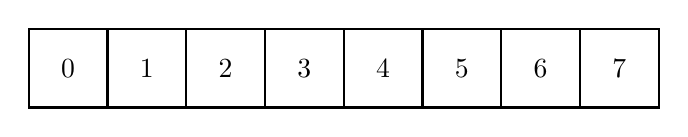
\begin{tikzpicture}
\draw[thick] (0,0) rectangle (1,1) node[midway] {0};
\draw[thick] (1,0) rectangle (2,1) node[midway] {1};
\draw[thick] (2,0) rectangle (3,1) node[midway] {2};
\draw[thick] (3,0) rectangle (4,1) node[midway] {3};
\draw[thick] (4,0) rectangle (5,1) node[midway] {4};
\draw[thick] (5,0) rectangle (6,1) node[midway] {5};
\draw[thick] (6,0) rectangle (7,1) node[midway] {6};
\draw[thick] (7,0) rectangle (8,1) node[midway] {7};
\end{tikzpicture}
\end{center}

\newpage

\section{Matrix}

\subsection{Definition}
A matrix is a 2D array, typically organized in rows and columns. Matrices are commonly used in mathematical computations, including linear algebra and graph theory. Each element in a matrix can be accessed by a pair of indices: the row and column numbers.

\subsection{Main Operations}
\begin{itemize}
    \item \textbf{Access:} Access an element using row and column indices.\\
    Time Complexity: $O(1)$
    
    \item \textbf{Insert:} Insert a new row or column in the matrix, which requires shifting elements.\\
    Time Complexity: $O(m \times n)$ (where $m$ and $n$ are the dimensions of the matrix)
    
    \item \textbf{Delete:} 
    \begin{itemize}
        \item If implemented as a static 2D array, removing a row or column requires shifting elements, leading to a time complexity of $O(m \times n)$. 
        \item If implemented as a vector of vectors, removing a row is simpler because each row is an independent vector. Removing a row involves removing a single element from the outer vector, making it $O(m)$, where $m$ is the number of rows.
    \end{itemize}

    \item \textbf{Search:} Find an element in the matrix by value.\\
    Time Complexity: $O(m \times n)$
    
    \item \textbf{Transpose:} Flip the matrix over its diagonal (row $i$ becomes column $i$).\\
    Time Complexity: $O(m \times n)$
\end{itemize}

\subsection{Diagram}
\begin{center}
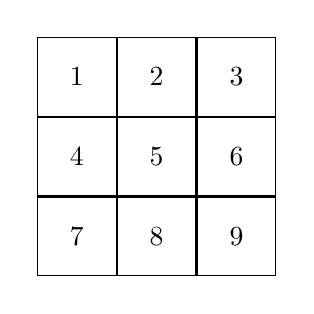
\begin{tikzpicture}
\matrix (m) [matrix of nodes,nodes in empty cells,
  nodes={draw, minimum size=1cm, anchor=center}] {
    1 & 2 & 3 \\
    4 & 5 & 6 \\
    7 & 8 & 9 \\
};
\end{tikzpicture}
\end{center}

\newpage

\section{Set}

\subsection{Definition}
A set is an unordered collection of distinct elements. Unlike arrays or matrices, sets do not allow duplicate values. They are commonly used to represent collections where each element is unique.

\subsection{Main Operations}
\begin{itemize}
    \item \textbf{Insert:} Add a new element to the set.\\
    Time Complexity: $O(1)$ on average (if implemented using a hash set), $O(\log n)$ if using a balanced binary tree.
    
    \item \textbf{Delete:} Remove an element from the set.\\
    Time Complexity: $O(1)$ on average (if using a hash set), $O(\log n)$ for a balanced binary tree.
    
    \item \textbf{Search (Contains):} Check if an element is present in the set.\\
    Time Complexity: $O(1)$ on average (hash set), $O(\log n)$ for a balanced binary tree.
    
    \item \textbf{Union:} Combine two sets into a single set containing all elements from both.\\
    Time Complexity: $O(n + m)$ (where $n$ and $m$ are the sizes of the sets).
    
    \item \textbf{Intersection:} Find elements that are present in both sets.\\
    Time Complexity: $O(\min(n, m))$
    
    \item \textbf{Difference:} Find elements in one set that are not in another.\\
    Time Complexity: $O(\min(n, m))$
\end{itemize}

\subsection{Diagram}
\begin{center}
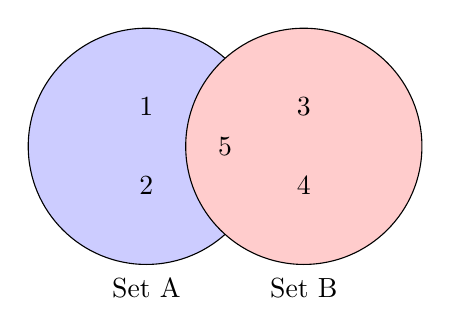
\begin{tikzpicture}
    \draw[fill=blue!20] (-1,0) circle (1.5cm) node at (-1,-1.8) {Set A};
    \draw[fill=red!20] (1,0) circle (1.5cm) node at (1,-1.8) {Set B};
    \node at (-1,0.5) {1};
    \node at (-1,-0.5) {2};
    \node at (1,0.5) {3};
    \node at (1,-0.5) {4};
    \node at (0,0) {5};
\end{tikzpicture}
\end{center}

\newpage

\section{Hash Table}

\subsection{Definition}
A hash table (or hash map) is a data structure that implements an associative array, a structure that can map keys to values. It uses a hash function to compute an index (or hash code) into an array of buckets, from which the desired value can be found. The main advantage of hash tables is their average time complexity for basic operations like insert, delete, and search, which is $O(1)$, assuming a good hash function and low collision rate.

\subsection{Main Operations}
\begin{itemize}
    \item \textbf{Insert:} Add a key-value pair to the hash table. If the key already exists, the value is updated.\\
    Time Complexity: $O(1)$ on average, but $O(n)$ in the worst case if too many collisions occur.

    \item \textbf{Delete:} Remove a key-value pair from the hash table. The hash function is used to locate the index of the key to remove.\\
    Time Complexity: $O(1)$ on average, but $O(n)$ in the worst case due to collisions.

    \item \textbf{Search:} Find a value by its associated key. The hash function computes the index, and the value is retrieved from that location.\\
    Time Complexity: $O(1)$ on average, but $O(n)$ in the worst case.

    \item \textbf{Collision Handling:} Since different keys can produce the same hash code (a collision), hash tables must handle collisions. Common methods include:
    \begin{itemize}
        \item \textbf{Chaining:} Each bucket points to a linked list of elements with the same hash value.
        \item \textbf{Open Addressing:} If a collision occurs, the algorithm looks for the next available slot.
    \end{itemize}
\end{itemize}

\subsection{Diagram}
\begin{center}
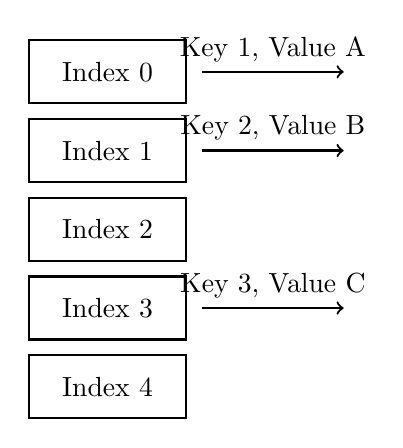
\begin{tikzpicture}
\draw[thick] (0,0) rectangle (2,0.8) node[midway] {Index 0};
\draw[thick] (0,-1) rectangle (2,-0.2) node[midway] {Index 1};
\draw[thick] (0,-2) rectangle (2,-1.2) node[midway] {Index 2};
\draw[thick] (0,-3) rectangle (2,-2.2) node[midway] {Index 3};
\draw[thick] (0,-4) rectangle (2,-3.2) node[midway] {Index 4};
\draw[->, thick] (2.2,0.4) -- (4,0.4) node[midway, above] {Key 1, Value A};
\draw[->, thick] (2.2,-0.6) -- (4,-0.6) node[midway, above] {Key 2, Value B};
\draw[->, thick] (2.2,-2.6) -- (4,-2.6) node[midway, above] {Key 3, Value C};
\end{tikzpicture}
\end{center}

\subsection{Advantages and Disadvantages}
\begin{itemize}
    \item \textbf{Advantages:}
    \begin{itemize}
        \item Fast average time complexity for search, insert, and delete operations ($O(1)$).
        \item Can store a large number of key-value pairs efficiently.
    \end{itemize}
    
    \item \textbf{Disadvantages:}
    \begin{itemize}
        \item Performance degrades if there are many collisions, leading to $O(n)$ complexity in the worst case.
        \item Requires a good hash function to minimize collisions.
    \end{itemize}
\end{itemize}


\end{document}
